% =============================================================================
% 绳驱折纸灵巧手仿真软件 Synergy Hand Simulator 架构设计
% 博士论文 - 软件系统章节
% 编译: xelatex software_architecture.tex
% =============================================================================
\documentclass[12pt,a4paper,openany]{book}

% ─── 中文支持 ───
\usepackage{fontspec}
\usepackage{xeCJK}
\setCJKmainfont{SimSun}[BoldFont=SimHei, ItalicFont=FangSong]
\setmainfont{Times New Roman}
\setsansfont{Arial}

% ─── 页面设置 ───
\usepackage[top=2.5cm, bottom=2.5cm, left=3cm, right=2.5cm]{geometry}
\usepackage{setspace}
\onehalfspacing

% ─── 数学公式 ───
\usepackage{amsmath, amssymb, amsthm}
\usepackage{bm}

% ─── 图形 ───
\usepackage{graphicx}
\usepackage{subcaption}
\usepackage{float}
\graphicspath{{figures/}}

% ─── 表格 ───
\usepackage{booktabs}
\usepackage{longtable}
\usepackage{array}
\usepackage{tabularx}

% ─── 代码列表 ───
\usepackage{listings}
\usepackage{xcolor}
\lstset{
    basicstyle=\small\ttfamily,
    columns=fullflexible,
    frame=single,
    breaklines=true,
    backgroundcolor=\color{gray!5},
    xleftmargin=2em,
    xrightmargin=2em,
}

% ─── 超链接 ───
\usepackage[colorlinks=true, linkcolor=black, citecolor=blue]{hyperref}

% ─── 引用样式 ───
\usepackage[numbers,sort&compress]{natbib}

% ─── 标题 ───
\usepackage{titlesec}
\titleformat{\chapter}{\centering\Large\bfseries}{第\,\thechapter\,章}{1em}{}
\titleformat{\section}{\large\bfseries}{\thesection}{1em}{}

% ─── 其他 ───
\usepackage{caption}
\usepackage{enumitem}
\usepackage{multirow}

\begin{document}

\chapter{绳驱折纸灵巧手仿真软件系统架构}

\section{引言}

绳驱折纸灵巧手（Cable-Driven Origami Hand）是一种基于折纸结构的新型柔性夹爪，其核心思想是利用折纸结构的屈曲折叠来模拟生物手指的关节运动，并通过腱绳传动实现多关节协同驱动。为了支持这类新型灵巧手的快速原型设计、运动学分析、协同控制算法验证以及物理仿真，我们开发了 \texttt{Synergy Hand Simulator} —— 一个面向折纸灵巧手的集成化仿真软件平台。

本章旨在系统性地介绍该软件的整体架构设计、核心模块功能、典型工作流程以及各模块间的数据交互关系。

\subsection{设计目标}

该仿真平台的开发遵循以下核心设计目标：

\begin{enumerate}[leftmargin=*,itemindent=0pt]
    \item \textbf{全流程覆盖}：从 DXF 图纸解析、拓扑结构重建、URDF 导出，到物理仿真和协同控制，提供端到端工具链支持。
    \item \textbf{模块化与可扩展性}：各功能模块解耦设计，便于独立开发和测试。更换运动学引擎不应影响 URDF 导出模块。
    \item \textbf{多物理引擎支持}：同时支持 MuJoCo（物理精确仿真）和 Pinocchio（实时运动学计算），满足不同场景需求。
    \item \textbf{交互式调试}：提供图形化用户界面，支持折痕选中、关节角度实时调节和 3D 可视化反馈，降低调试门槛。
    \item \textbf{协同控制验证}：原生集成自适应协同（Adaptive Synergy）、增强自适应协同（Augmented Adaptive Synergy）和动态协同（Dynamic Synergy）三种控制模型。
\end{enumerate}

\section{系统总体架构}

系统采用分层设计，自顶向下分为四层：数据输入层、核心模型层、协同控制层和仿真交互层。图~\ref{fig:architecture} 展示了各层间的依赖关系和数据流。

\begin{figure}[H]
    \centering
    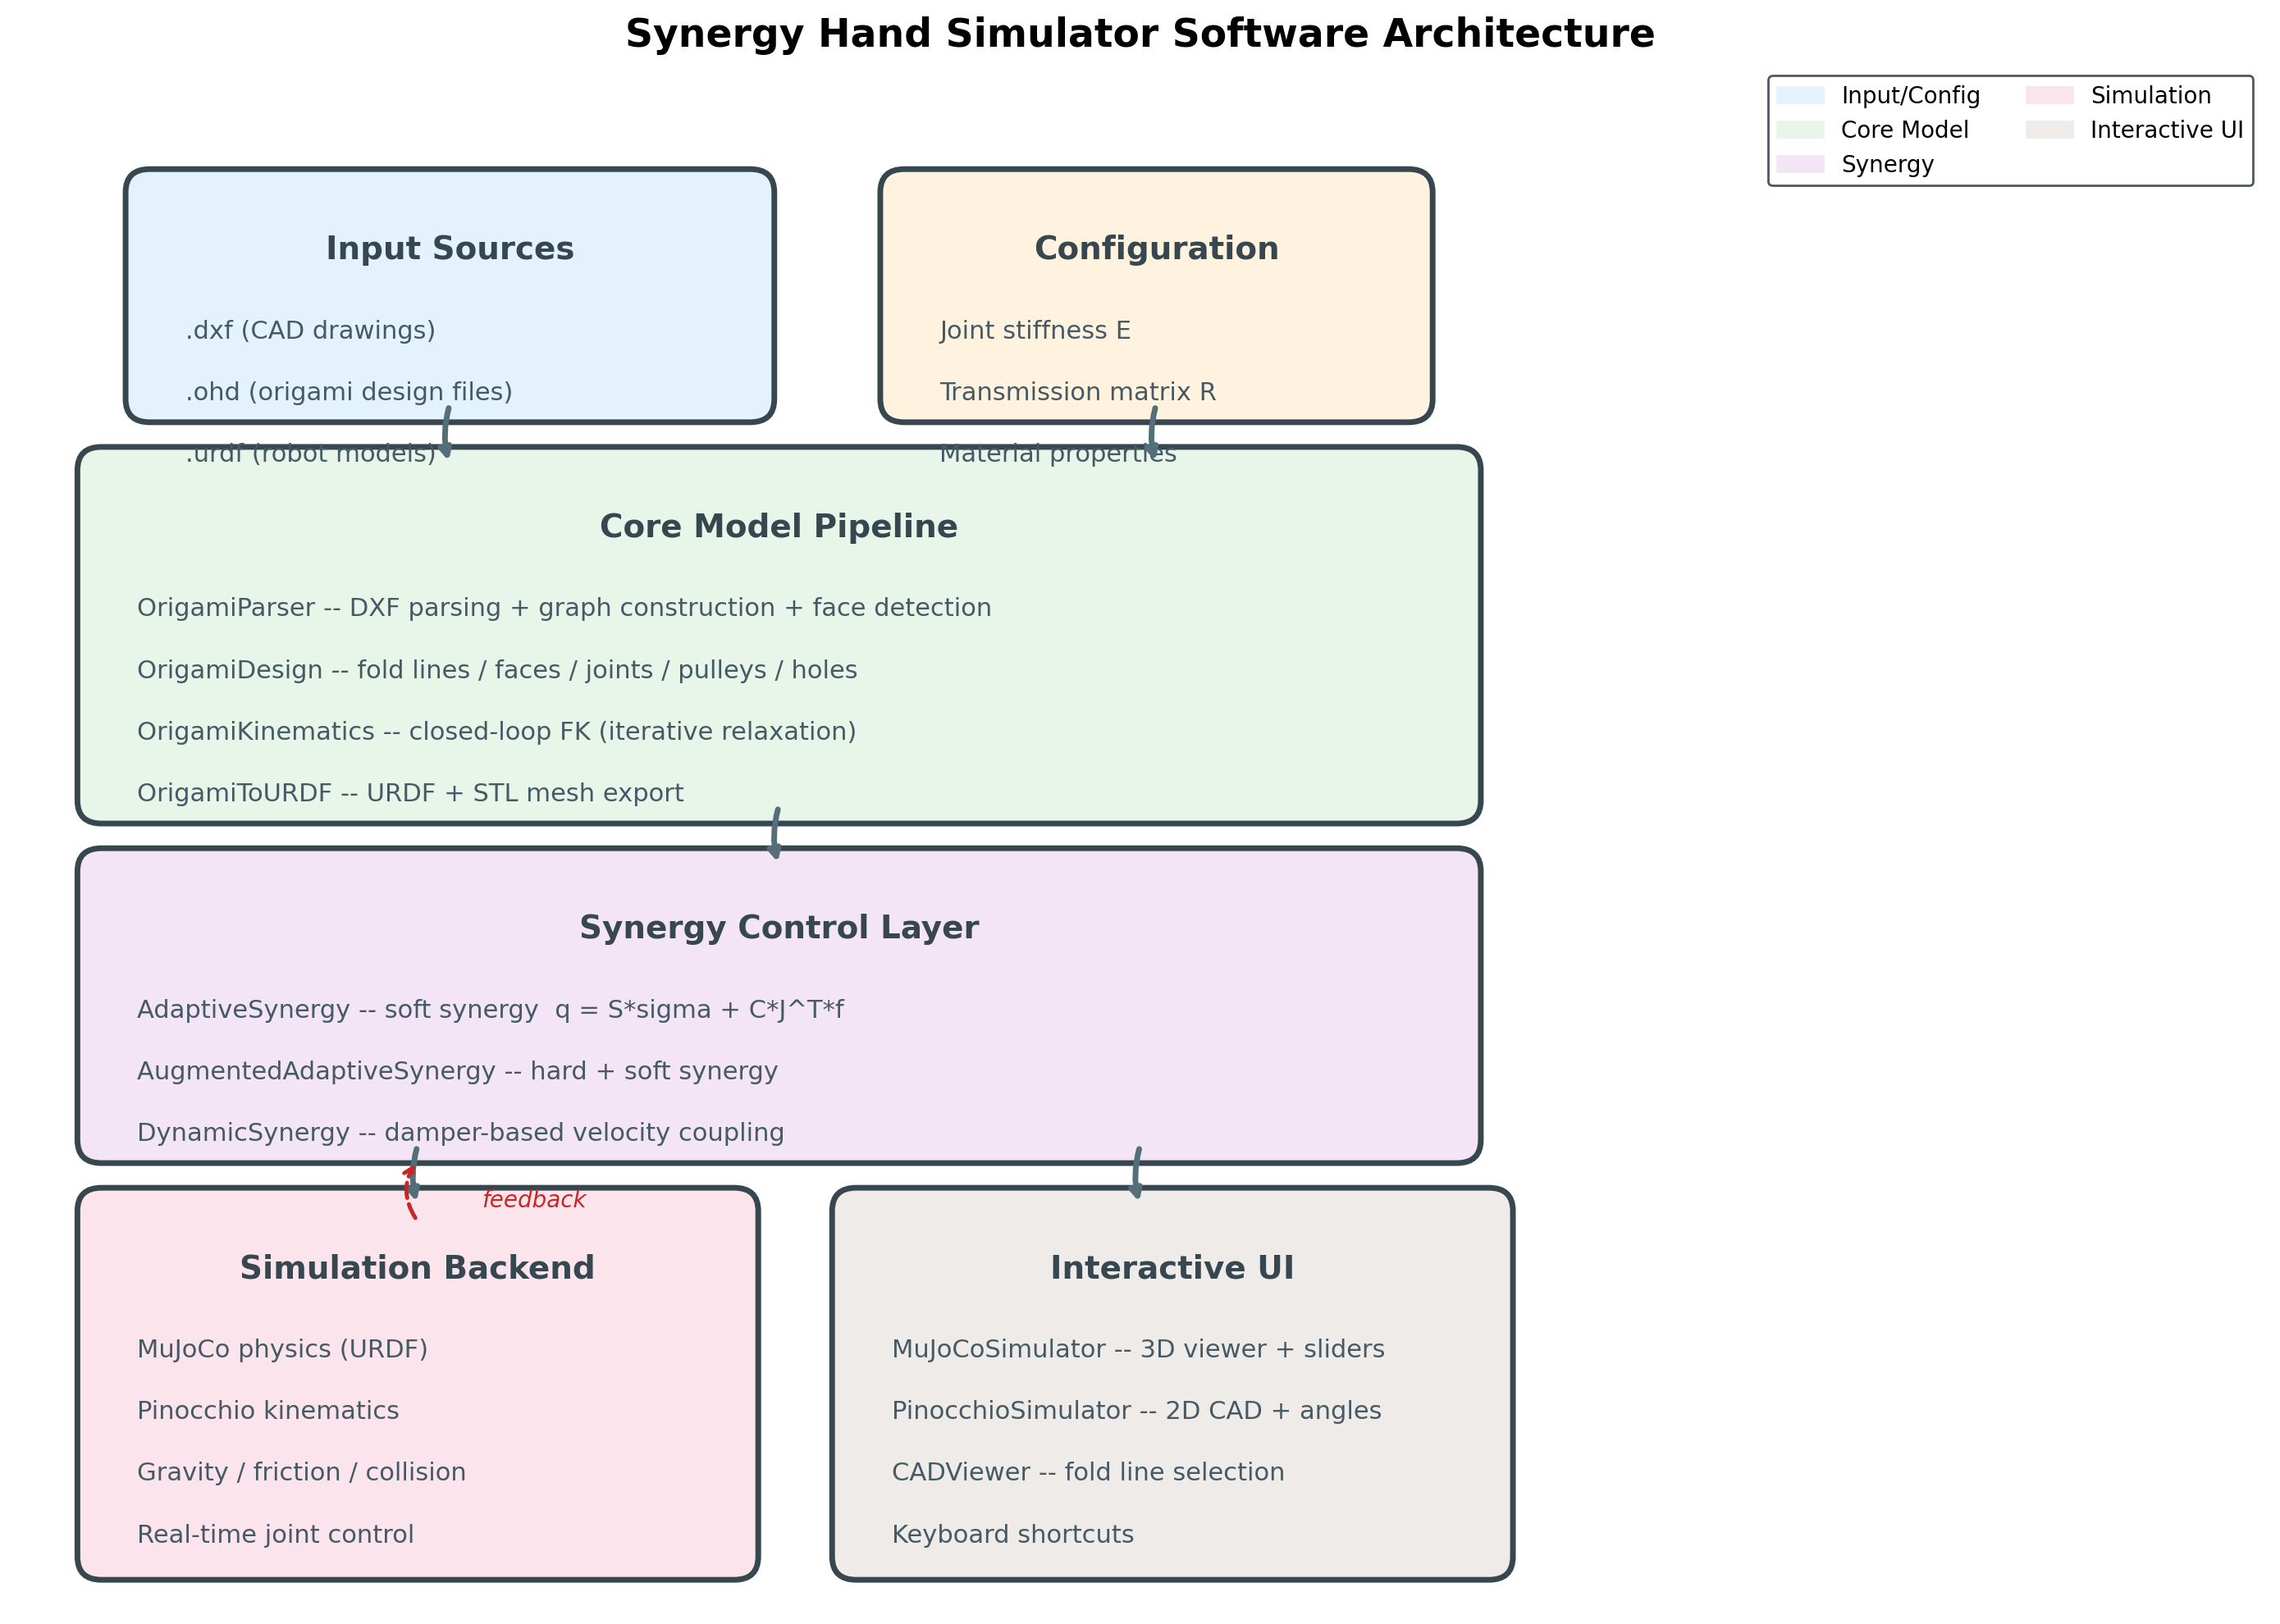
\includegraphics[width=\textwidth]{architecture.png}
    \caption{Synergy Hand Simulator 系统架构图。各层之间通过标准化数据接口交互。}
    \label{fig:architecture}
\end{figure}

\subsection{数据输入层}

数据输入层位于系统最上层，负责接收和解析外部模型数据，支持三种格式：

\begin{itemize}
    \item \textbf{DXF 格式}：AutoCAD 的标准交换格式。用户可在 CAD 软件中绘制折纸手的 2D 展开图，以不同图层颜色区分峰折（红色）、谷折（蓝色）和轮廓线（黑色）。
    \item \textbf{OHD 格式}：自定义折纸手设计文件（Origami Hand Design），以 JSON 格式保存完整的折痕线、面片、关节、滑轮、孔和腱绳路径等结构化信息。
    \item \textbf{URDF 格式}：机器人描述格式标准。可通过系统自带的 \texttt{OrigamiToURDF} 模块从 DXF 或 OHD 导出，也可直接加载兼容 URDF 的模型。
\end{itemize}

用户还需通过配置文件指定关节刚度向量 \( \bm{E} \) 和传动矩阵 \( \bm{R} \)，这两个参数是后续协同控制计算的输入基础。

\subsection{核心模型层}

核心模型层是系统的几何和运动学引擎，包含四个模块：

\begin{enumerate}
    \item \texttt{OrigamiParser}（折纸解析器）：读取 DXF 文件中线段实体，根据颜色索引识别折痕类型。核心算法包括线段分割（交点处断开）、无向图构建、面片搜索（最小环路算法）和外轮廓剔除，最终输出 \texttt{OrigamiHandDesign} 对象。
    \item \texttt{OrigamiDesign}（折纸设计）：数据模型核心容器，使用 \texttt{FoldLine}、\texttt{OrigamiFace}、\texttt{JointConnection}、\texttt{Pulley}、\texttt{Hole}、\texttt{Damper}、\texttt{Tendon} 等数据类（dataclass）描述折纸手的几何拓扑、传动系统和弹性特性，支持 \texttt{to\_dict}/\texttt{from\_dict} 序列化。
    \item \texttt{OrigamiKinematics}（折纸运动学）：实现折纸结构正向运动学。使用迭代约束松弛法处理闭环运动学——先沿生成树传播变换，再逐次修正环闭合误差。关节角度物理限位：谷折范围为 \([0, \pi]\)，山折范围为 \([-\pi, 0]\)。
    \item \texttt{OrigamiToURDF}（URDF 导出）：将折纸设计转换为 URDF 格式和 STL 三角网格文件。自动处理峰谷折痕分层定位——谷折关节轴位于父面片上表面（\(z=0\)），峰折位于下表面（\(z=-t\)，\(t\) 为板材厚度），并确定正确的旋转轴方向。
\end{enumerate}

\subsection{协同控制层}

协同控制层是系统的智能核心。图~\ref{fig:synergy_model} 展示了基础自适应协同模型的数学原理。

\begin{figure}[H]
    \centering
    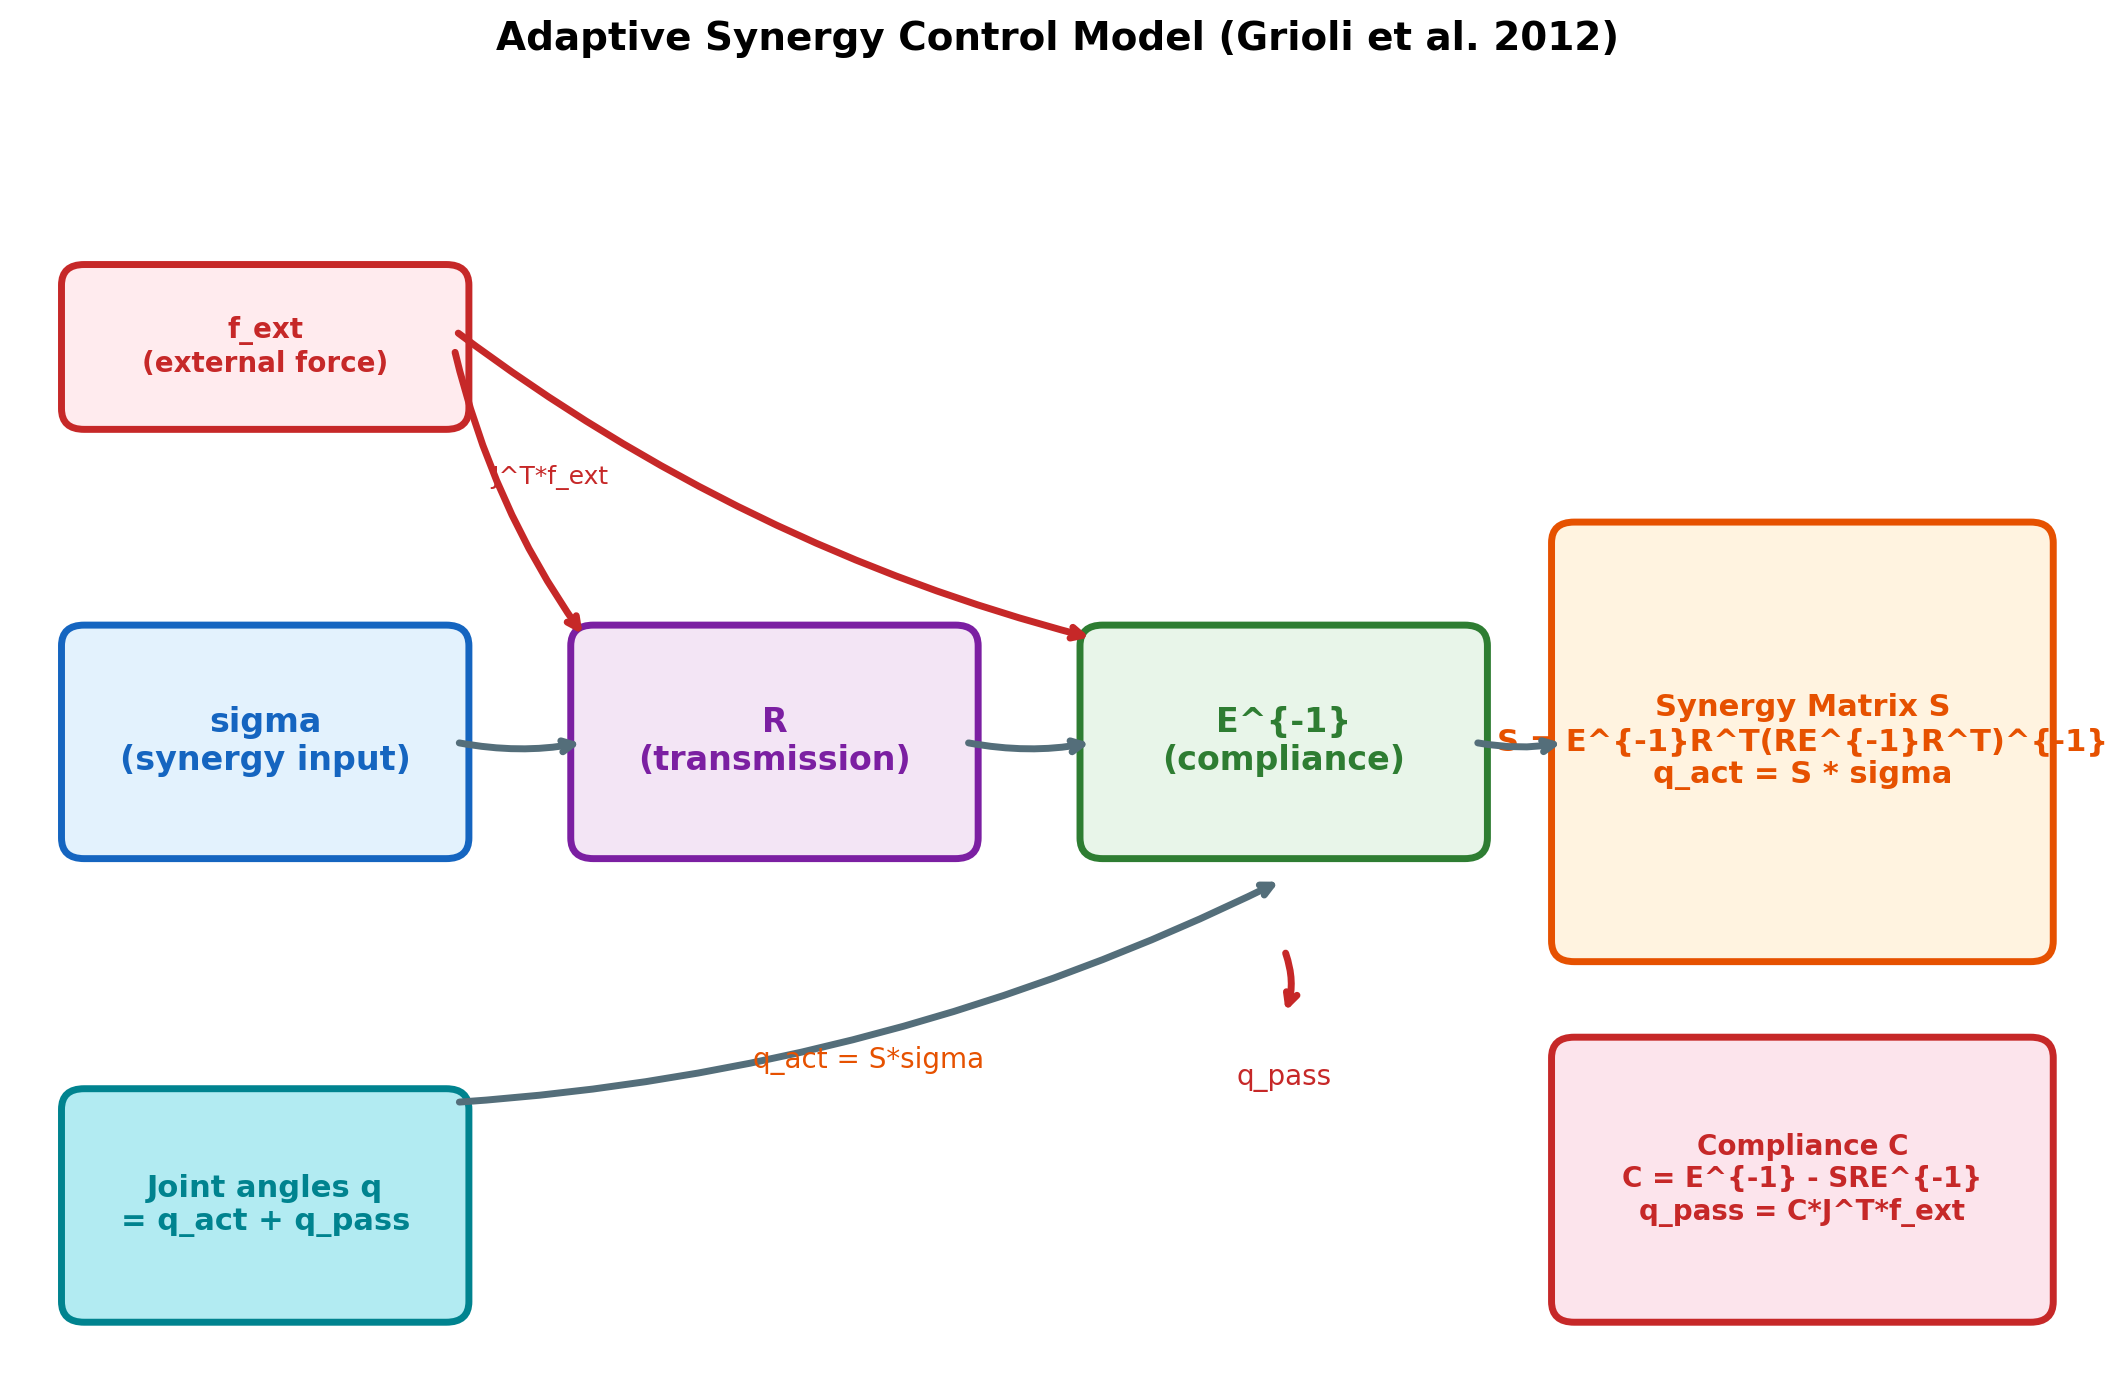
\includegraphics[width=0.85\textwidth]{synergy_model.png}
    \caption{自适应协同控制模型示意图。协同输入 \(\sigma\) 经传动矩阵 \(\bm{R}\) 和柔顺矩阵 \(\bm{E}^{-1}\) 形成主动协同矩阵 \(\bm{S}\)，驱动关节运动；外力 \(\bm{f}_{\text{ext}}\) 通过 \(\bm{C}\) 产生被动偏移。}
    \label{fig:synergy_model}
\end{figure}

\begin{enumerate}
    \item \textbf{AdaptiveSynergyModel}（自适应协同）：基于 Grioli 等人\cite{grioli2012adaptive}提出的软协同理论，通过传动矩阵 \(\bm{R} \in \mathbb{R}^{k \times n}\) 将 \(k\) 个协同输入 \(\bm{\sigma}\) 映射到 \(n\) 个关节角度 \(\bm{q}\)：
    \begin{align}
        \bm{S} &= \bm{E}^{-1} \bm{R}^{\mathsf{T}} (\bm{R} \bm{E}^{-1} \bm{R}^{\mathsf{T}})^{-1}, \\
        \bm{C} &= \bm{E}^{-1} - \bm{S} \bm{R} \bm{E}^{-1}, \\
        \bm{q} &= \bm{S} \bm{\sigma} + \bm{C} \bm{J}^{\mathsf{T}} \bm{f}_{\text{ext}}.
    \end{align}
    其中 \(\bm{E}\) 为对角关节刚度矩阵，\(\bm{S}\) 和 \(\bm{C}\) 分别为主动协同矩阵与被动柔顺矩阵，\(\bm{J}\) 为抓取雅可比矩阵，\(\bm{f}_{\text{ext}}\) 为外力旋量。
    
    \item \textbf{AugmentedAdaptiveSynergyModel}（增强自适应协同）：在软协同基础上增加硬协同约束。硬协同通过机械联动实现确定的关节耦合，软协同允许在外力作用下偏离协同轨迹，适用于需要兼顾精确传动和被动柔顺的设计。
    
    \item \textbf{DynamicSynergyModel}（动态协同）：引入阻尼器元件实现速度相关耦合。阻尼位移 \(\bm{x} = \bm{T} \bm{q}\)，阻尼力 \(-c \dot{\bm{x}}\)，产生随速度变化的关节耦合效果，适用于动态调节抓取刚度的场景。
\end{enumerate}

\subsection{仿真交互层}

仿真交互层承担物理仿真和用户交互的双重职责：

\begin{itemize}
    \item \textbf{MuJoCoSimulator}：基于 MuJoCo 物理引擎的 3D 仿真器。支持 URDF 加载、重力/摩擦物理属性、碰撞检测和实时关节驱动。提供 3D 查看器窗口和滑块面板，同时支持编程接口自动化控制。
    \item \textbf{PinocchioSimulator}：基于 Pinocchio 运动学库的轻量级仿真器。提供 2D CAD 视图和角度控制面板，用户可通过点击折痕线（山折/谷折以▲/▼标记）选中关节，使用滑块或键盘快捷键（↑/↓ 步进5°，←/→ 步进1°）微调。
    \item \textbf{CADViewer}：2D 折纸展开图查看器，支持折痕线可视化分类显示和点击选取，是 PinocchioSimulator 的重要组件。
\end{itemize}

\section{软件工作流}

图~\ref{fig:workflow} 展示典型使用流程，覆盖从设计输入到仿真验证的完整闭环。

\begin{figure}[H]
    \centering
    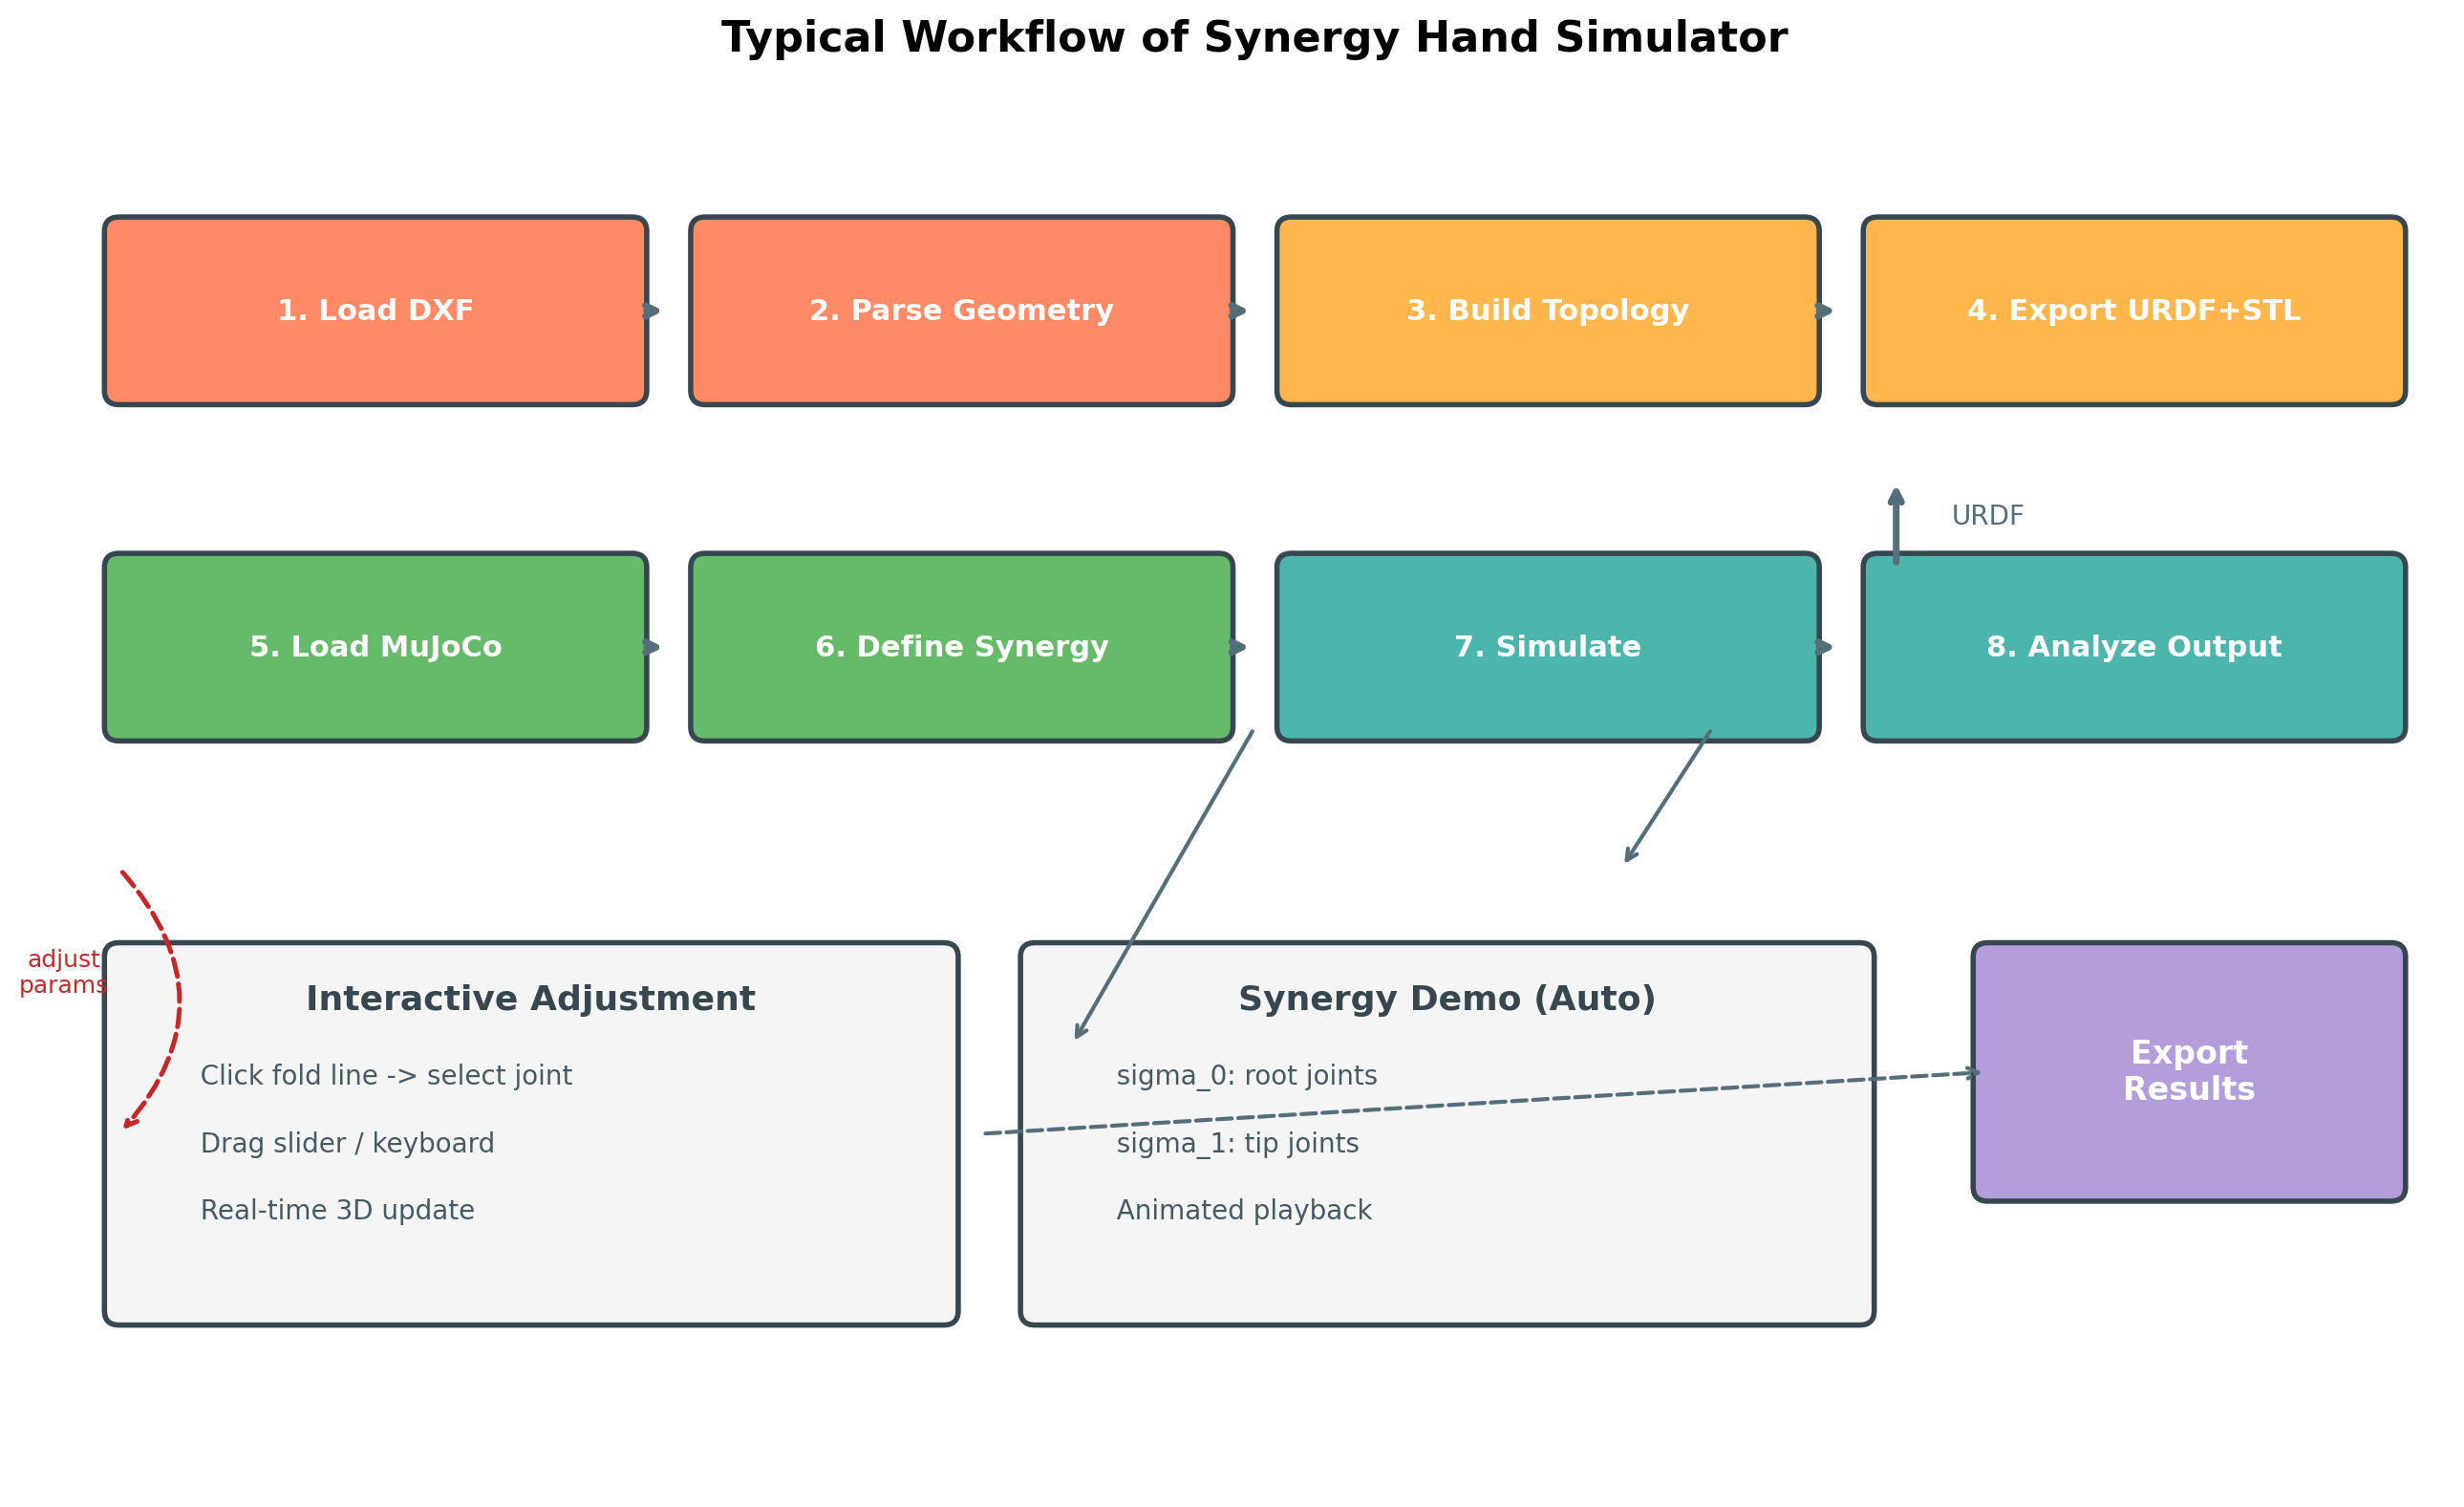
\includegraphics[width=\textwidth]{workflow.png}
    \caption{典型工作流程图。流程包括：加载 DXF → 几何解析 → 拓扑重建 → URDF 导出 → 加载仿真器 → 定义协同参数 → 仿真/调试 → 输出结果。}
    \label{fig:workflow}
\end{figure}

具体操作步骤如下：

\begin{enumerate}
    \item \textbf{设计输入}：在 CAD 软件中绘制折纸手 2D 展开图，红色为峰折、蓝色为谷折、黑色为轮廓线，导出 DXF 格式。
    \item \textbf{几何解析}：运行 \texttt{scripts/export\_urdf.py}，调用 \texttt{OrigamiParser} 解析 DXF，自动识别面片和关节拓扑。
    \item \textbf{URDF 导出}：\texttt{OrigamiToURDF} 自动生成 STL 网格和 URDF 描述文件，导出至 \texttt{models/<hand\_name>/} 目录。
    \item \textbf{仿真加载}：启动 MuJoCo 或 Pinocchio 仿真器加载生成的 URDF，例如：\texttt{python scripts/run\_mujoco\_simulator.py models/test\_3/test\_3.urdf}。
    \item \textbf{协同控制}：编写协同控制脚本（如 \texttt{scripts/synergy\_mujoco\_demo.py}），定义 \(\bm{R}\) 和 \(\bm{E}\)，使用 \texttt{AdaptiveSynergyModel.solve()} 计算协同关节角并驱动仿真。
    \item \textbf{交互调试}：通过 GUI 面板或快捷键实时调整关节角度，观察 3D 模型运动响应，迭代优化协同参数。
    \item \textbf{结果输出}：将调试好的协同参数导出，用于实际硬件控制。
\end{enumerate}

\section{代码模块组织}

系统源代码按功能划分为五个子包，图~\ref{fig:modules} 展示了模块间依赖关系。

\begin{figure}[H]
    \centering
    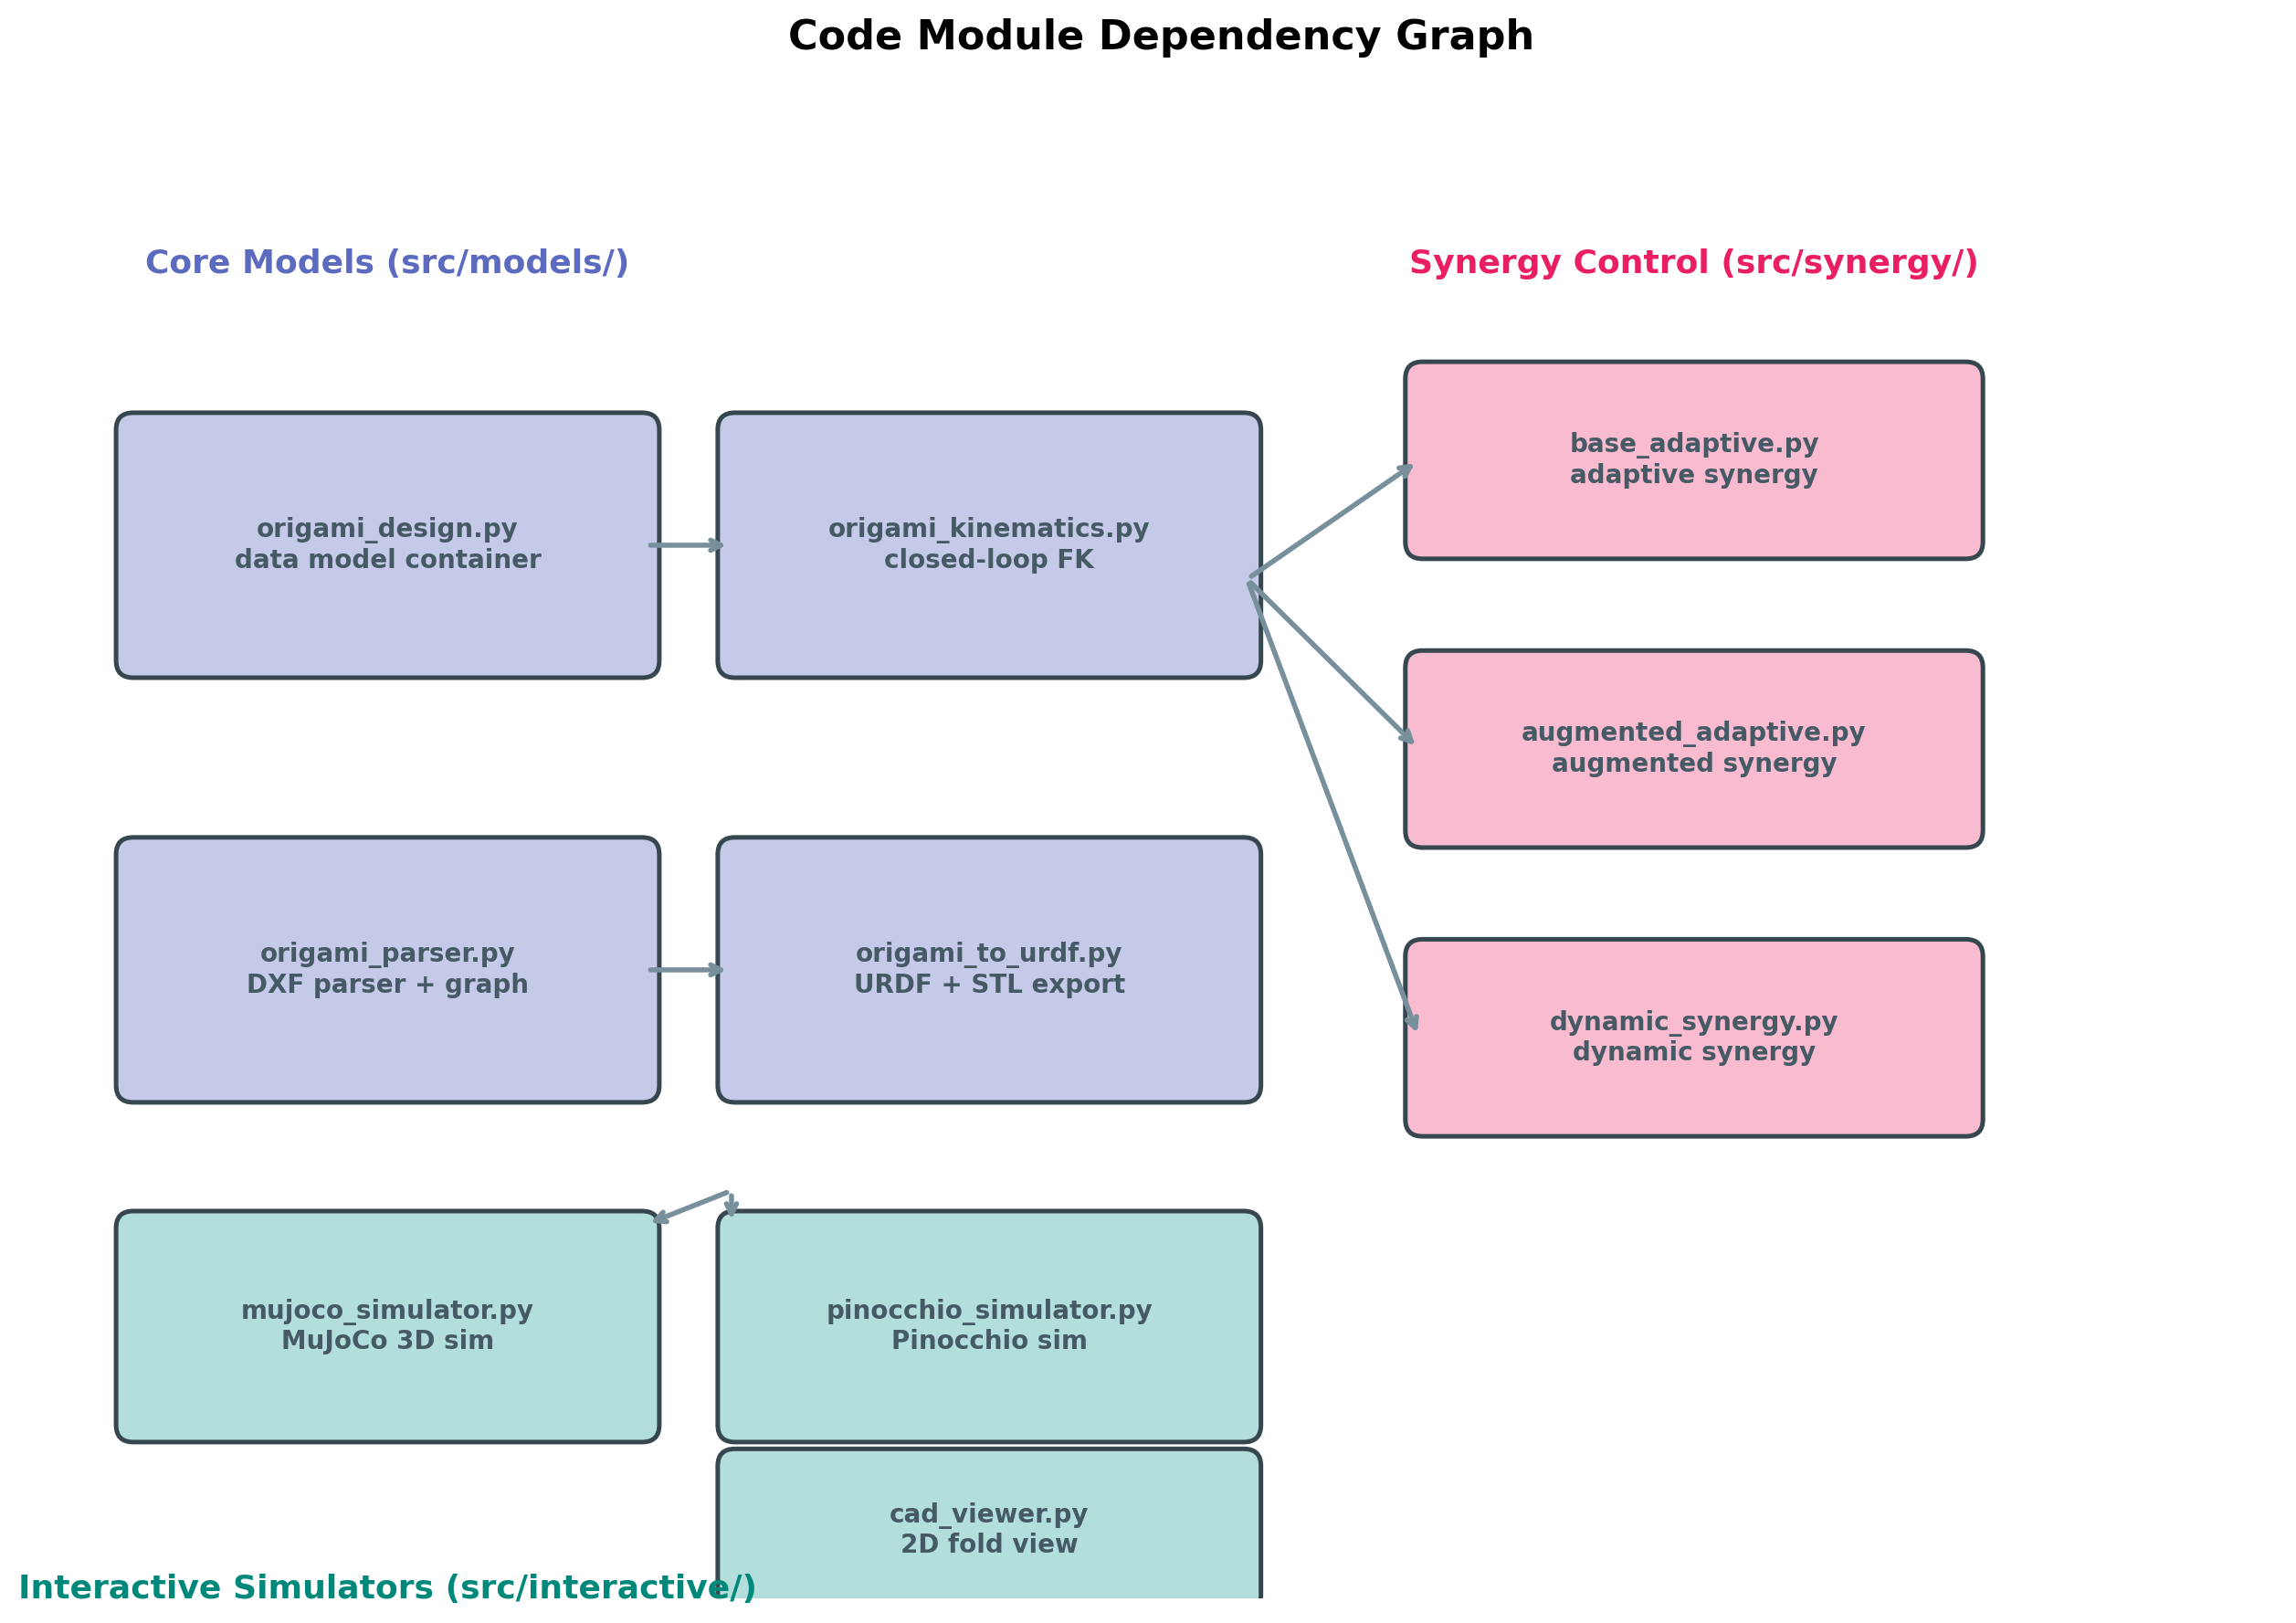
\includegraphics[width=\textwidth]{modules.png}
    \caption{代码模块依赖图。展示了三大核心包 \texttt{src/models/}、\texttt{src/synergy/}、\texttt{src/interactive/} 之间的调用关系。}
    \label{fig:modules}
\end{figure}

各子包的核心职责和关键文件如表~\ref{tab:modules} 所示。

\begin{table}[H]
    \centering
    \caption{代码模块一览}
    \label{tab:modules}
    \small
    \begin{tabularx}{\textwidth}{p{2.5cm}p{2.5cm}X}
    \toprule
    \textbf{子包} & \textbf{核心文件} & \textbf{主要功能} \\
    \midrule
    \texttt{src/models/} & \texttt{origami\_design.py} & 数据模型定义（折痕线、面片、关节、滑轮、孔等） \\
    & \texttt{origami\_parser.py} & DXF 解析、平面图构建、面片识别 \\
    & \texttt{origami\_kinematics.py} & 正向运动学（含闭环约束松弛） \\
    & \texttt{origami\_to\_urdf.py} & URDF/STL 导出 \\
    \midrule
    \texttt{src/synergy/} & \texttt{base\_adaptive.py} & 自适应协同模型 \\
    & \texttt{augmented\_adaptive.py} & 增强自适应协同 \\
    & \texttt{dynamic\_synergy.py} & 动态协同模型 \\
    \midrule
    \texttt{src/interactive/} & \texttt{mujoco\_simulator.py} & MuJoCo 3D 仿真界面 \\
    & \texttt{pinocchio\_simulator.py} & Pinocchio 运动学仿真界面 \\
    & \texttt{cad\_viewer.py} & 2D CAD 折痕视图 \\
    \midrule
    \texttt{scripts/} & \texttt{export\_urdf.py} & DXF$\rightarrow$URDF 导出入口 \\
    & \texttt{run\_mujoco\_simulator.py} & MuJoCo 仿真启动入口 \\
    & \texttt{run\_pinocchio\_simulator.py} & Pinocchio 仿真启动入口 \\
    & \texttt{synergy\_mujoco\_demo.py} & 协同驱动 MuJoCo 演示 \\
    \midrule
    \texttt{tests/} & \texttt{test\_origami\_kinematics.py} & 运动学单元测试 \\
    & \texttt{test\_adaptive\_synergy.py} & 自适应协同单元测试 \\
    & \texttt{test\_augmented\_synergy.py} & 增强协同单元测试 \\
    \bottomrule
    \end{tabularx}
\end{table}

\section{关键技术细节}

\subsection{折痕线与关节映射}

折纸结构的核心特征在于：一条折痕线在 2D 展开图中是线段，在 3D 折叠状态下成为旋转关节。\texttt{JointConnection} 数据结构记录每条折痕两侧相邻面片（\texttt{face\_a\_id} 和 \texttt{face\_b\_id}）以及折痕类型。关节旋转轴方向为折痕线在 2D 平面中的方向向量，轴位置位于折痕中点。峰折与谷折的区别在于板材偏移方向：谷折关节轴在板上表面（\(z=0\)），峰折在下表面（\(z=-t\)，板材厚度 \(t=3\)mm）。

\subsection{拓扑重建算法}

\texttt{build\_topology()} 方法是折纸设计管线的核心。其输入为初始折痕线集合（可能存在交叉），输出为结构化的面片-关节拓扑。算法步骤包括：(1) 线段交点处分割（\texttt{split\_at\_intersections}），确保图为严格平面图；(2) 建立无向图（\texttt{build\_graph\_from\_segments}），记录节点坐标和边类型；(3) 最小环路算法（\texttt{find\_minimal\_cycles}）搜索基本环路，每环对应一个折纸面片；(4) 剔除最大面积外轮廓面（\texttt{remove\_outer\_face}）；(5) 基于边-面映射重建关节连接。

拓扑重建后，原先附加在折痕线上的孔和滑轮元素的 \texttt{attached\_fold\_line\_id} 会失效。修复策略为：根据这些元素的几何位置，自动寻找最近的谷折或峰折折痕线重新挂载。

\subsection{闭环运动学求解}

折纸结构天然存在闭环。\texttt{OrigamiForwardKinematics} 采用迭代约束松弛法处理：首先生成以根面片为根的面片生成树，沿树传播旋转变换；然后检测环边上的位置和方向误差，若超过容差（\(10^{-6}\)），则将误差分配到相关路径关节角度中，重复迭代直至收敛。

各关节旋转使用 Rodrigues 公式：
\[
\bm{R}(\bm{\omega}, \theta) = \bm{I} + \sin\theta [\bm{\omega}]_\times + (1 - \cos\theta) [\bm{\omega}]_\times^2,
\]
其中 \(\bm{\omega}\) 为归一化旋转轴方向，\(\theta\) 为关节角度。

\subsection{协同矩阵的计算稳定性}

\texttt{AdaptiveSynergyModel} 中关键数值细节是对伪逆（pinv）的使用：

\begin{lstlisting}[language=Python, caption={自适应协同模型预计算核心代码}]
E_inv = np.diag(1.0 / np.diag(self.E))
RE = self.R @ E_inv @ self.R.T
RE_inv = np.linalg.pinv(RE)       # 伪逆而非普通逆
self.S = E_inv @ self.R.T @ RE_inv
self.C = E_inv - self.S @ self.R @ E_inv
\end{lstlisting}

使用 \texttt{pinv} 而非 \texttt{inv} 的原因：当传动矩阵 \(\bm{R}\) 各行间共线时（如滑轮半径和摩擦系数相同），\(\bm{R} \bm{E}^{-1} \bm{R}^{\mathsf{T}}\) 可能秩亏缺。伪逆自动将零空间分量投影为零，同时保持非零空间分量的正确性，保证数值稳定性。

\section{本章小结}

本章详细介绍了 \texttt{Synergy Hand Simulator} 仿真平台的系统架构和软件设计。该平台涵盖折纸设计解析（DXF$\rightarrow$拓扑$\rightarrow$URDF）、仿真验证（MuJoCo/Pinocchio 双引擎）、协同控制（自适应/增强/动态三种模型）三大核心功能，提供从 CAD 设计到仿真验证的完整工具体系。

系统的模块化设计使各功能可独立开发、测试和复用。核心模型包 \texttt{src/models/} 不依赖任何 GUI 库，可在无图形界面的服务器环境下运行；协同控制层完全基于 NumPy，不依赖仿真引擎，可独立用于数值实验。这为后续硬件集成和算法扩展奠定了良好的软件基础。

\begin{thebibliography}{9}
\bibitem{grioli2012adaptive} G. Grioli, M. Catalano, E. Silvestro, S. Tono, and A. Bicchi, ``Adaptive synergies: an approach to the design of under-actuated robotic hands,'' in \textit{Proc. IEEE/RSJ IROS}, 2012, pp. 1251--1256.
\end{thebibliography}

\end{document}
